\chapter{Аналитический раздел}
\section{Анализ предметной области}

Ограниченный естественный язык – это подмножество естественного языка, текст на котором, без каких-либо усилий, воспринимается носителем исходного естественного языка, а также не требует длительного изучения для приобретения навыков составления текстов на этом языке, однако обладает сокращенным набором лексики и грамматики. Использование ограниченного естественного языка позволяет снизить время обработки естественно-языковых конструкций, без снижения уровня функциональности~\cite{Zhitko2011}. 

Разметка текста заключается в приписывании словам или предложениям меток (тэгов) в соответствии с характером разметки: морфологические, синтаксические, семантические и другие~\cite{Zaharov}.

Джеффри Лич приводит следующие принципы, которым должна подчиняться разметка общедоступного корпуса~\cite{Leech1997}:
\begin{itemize}
	\item разметка должна основываться на доступной для пользователя в виде руководства или инструкции схеме анализа, в которой должно быть мотивированно введение каждого параметра;
	\item разметка общедоступного корпуса должна опираться на общеизвестную систему правил и классификаций;
	\item должно быть ясно кто и как разрабатывает схему аннотации и каковы ограничения, например юридические или технические, при использовании корпусом~\cite{Kopotev}.
\end{itemize}

Синтаксическая разметка является результатом разбора, выполняемого на основе данных морфологического анализа. Данный вид разметки описывает синтаксические связи и конструкции, образованные лексическими единицами~\cite{Zaharov,Kopotev}. Тексты, получившие синтаксическую разметку известны в англоязычной литературе как treebanks~\cite{abeeille2003treebanks}. Пример визуализации синтаксических зависимостей, отображаемых синтаксической разметкой, представлен на рисунке~\ref{fig:syntax_annotation}.

\begin{figure}[H]
	\centering
	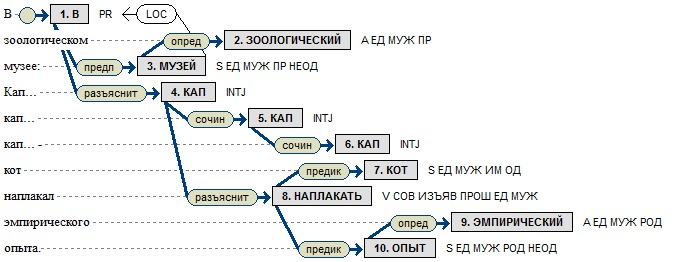
\includegraphics[width=0.9\linewidth]{images/syntax_annotation.png}
	\caption{Визуализация синтаксических зависимостей в НКРЯ}
	\label{fig:syntax_annotation}
\end{figure}

В корпусной лингвистике наблюдается большое разнообразие синтаксических теорий и формализмов, среди которых наиболее распространенными являются следующие~\cite{Zaharov,gladkij1985sintaksicheskie}:
\begin{itemize}
	\item системы зависимостей;
	\item системы непосредственных составляющих;
	\item системы синтаксических групп.
\end{itemize}


\section{Системы синтаксической разметки}
\subsection{Системы зависимостей}

Если \textit{П}~---~конечное линейное упорядоченное множество, то всякое дерево $D$, для которого \textit{П} служит множеством узлов, называется деревом синтаксического подчинения (зависимостей) на \textit{П}. Если \textit{П}~---~множество точек некоторой цепочки $x$, говорят, что $D$~---~дерево синтаксического подчинения (зависимостей) для $x$~\cite{gladkij1985sintaksicheskie}. Размеченным деревом подчинения(зависимостей) называется упорядоченная четверка~\ref{eq:marked_dep_tree}:
\begin{equation}
	\label{eq:marked_dep_tree}
	\langle\textit{П},\rightarrow,Z,\psi\rangle,
\end{equation}
\noindent\makebox[0pt][l]{где }\hspace*{\parindent}$\langle\textit{П}, \rightarrow\rangle$~---~дерево зависимостей на $\textit{П}$,
	
	$Z$~---~конечное множество меток,
	
	$\psi$~---~разметка, отображение множества дуг дерева в $Z$.

Таким образом дерево зависимостей представляет собой дерево, в котором вершины соответствуют отдельным словам предложения, а дуги между ними~---~синтаксическим подчинительным связям между словами~\cite{bolshakova2017avtomaticheskaya}. Пример дерева зависимостей для шведского языка приведен на рисунке~\ref{fig:dep_tree}.

\begin{figure}[H]
	\centering
	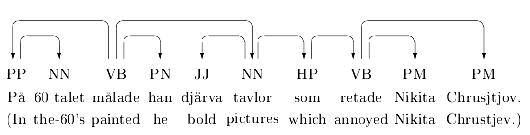
\includegraphics[width=0.7\linewidth]{images/dep_tree_swedish.png}
	\caption{Дерево зависимостей предложения на шведском языке}
	\label{fig:dep_tree}
\end{figure}

Дерево подчинения $\langle\textit{П}, \rightarrow\rangle$ называется проективным, если для любых трех его узлов $\alpha$, $\beta$, $\gamma$ из того, что $\alpha \rightarrow \beta$ и $\gamma$ лежит между $\alpha$ и $\beta$, следует, что $\gamma$ зависит от $\alpha$. Проективные предложения соответствуют <<естественному>> порядку слов, тогда как непроективные более характерны художественной литературе~\cite{gladkij1985sintaksicheskie}. Например, следующий оборот не является проективным: <<... рассмотрев выдвинутые здесь предложения товарищем Лопаткиным...>>.

Требование проективности исходного предложения и, как следствие, получаемого дерева зависимостей, является необходимым для большинства алгоритмов построения деревьев зависимостей. Алгоритм Нивре~\cite{nivre2003efficient}, являющийся основой MaltParser~\cite{nivre2007maltparser}, алгоритм, используемый в LPaRus~\cite{kiselev2017sintaksicheskij} также основываются на предположении, что предложение проективно.

Среди преимуществ систем зависимостей выделяют~\cite{gladkij1985sintaksicheskie,Testelets2001,nivre2003efficient}:
\begin{itemize}
	\item независимость от порядка слов в предложении;
	\item однозначность отношения <<главное--зависимое>> между словоформами.
\end{itemize}

Помимо требования проективности к недостаткам систем зависимостей относят~\cite{gladkij1985sintaksicheskie,Testelets2001,kiselev2017sintaksicheskij,Grashchenkov2024RuConst}:
\begin{itemize}
	\item невозможность отобразить связи и иерархию словосочетаний;
	\item невозможность в полной мере описать неподчинительные связи;
	\item неоднозначность определения управляющей словоформы в некоторых случаях;
	\item невозможность различить адъюнкты и аргументы при предикате.
\end{itemize}



\subsection{Системы составляющих}

Множество $C$ отрезков конечного линейно упорядоченного множества $\textit{П}$ называется системой составляющих на $\textit{П}$, если оно удовлетворяет следующим условиям~\cite{gladkij1985sintaksicheskie}:
\begin{enumerate}
	\item $C$ содержит в качестве элементов само $\textit{П}$ и все одноточечные отрезки $\textit{П}$;
	\item любые два отрезка из $C$ либо не пересекаются, либо один из них содержится в другом.
\end{enumerate}

Если $\textit{П}$~---~множество точек некоторой цепочки $x$, говорят о системе составляющих цепочки $x$~\cite{gladkij1985sintaksicheskie}. Пример неразмеченного дерева составляющих представлен на рисунке~\ref{fig:cons_tree}.

\begin{figure}[h!]
	\centering
	
\includegraphics[width=0.7\textwidth]{cons_tree_example.pdf}
	\caption{Неразмеченное дерево составляющих для предложения на русском языке}
	\label{fig:cons_tree}
\end{figure}

Размеченной системой составляющих называют упорядоченную тройку:
\begin{equation}
	\label{eq:marked_cons_tree}
	\langle C,W,\varphi\rangle,
\end{equation}
\noindent\makebox[0pt][l]{где }\hspace*{\parindent}$C$~---~система составляющих,

$W$~---~конечное множество меток,

$\varphi$~---~разметка, отображение $C$ в множество всех непустых подмножеств $W$.

Таким образом дерево составляющих представляет собой дерево, в котором в листьях находятся слова предложения, поддеревья соответствуют входящим в предложение синтаксическим конструкциям, а дуги выражают отношение вложенности конструкций~\cite{bolshakova2017avtomaticheskaya}. Пример размеченного дерева составляющих представлен на рисунке~\ref{fig:marked_cons_tree}.

\begin{figure}[h!]
	\centering
	
\includegraphics[width=0.5\textwidth]{marked_cons_tree.png}
	\caption{Размеченное дерево составляющих для предложения на русском языке}
	\label{fig:marked_cons_tree}
\end{figure}

К преимуществам системы составляющих относят~\cite{Testelets2001,Grashchenkov2024RuConst,jurafsky2026speech,Poletaev2023ConstituencyTree}:
\begin{itemize}
	\item явную разметку фразовых категорий и синтаксических единиц;
	\item учет грамматически правильного порядка слов;
	\item построение грамматики для работы алгоритма на основе типов составляющих, что является более общим подходом, чем части речи;
	\item возможность различить адъюнкты и аргументы при предикате;
	\item возможность описать правила сочинения составляющих;
	\item применимость построенных деревьев для дальнейшего семантического анализа;
	\item возможность использования полученных синтаксических единиц и групп для прикладных задач.
\end{itemize}

Основными недостатками систем составляющих являются~\cite{jurafsky2026speech,Testelets2001,bolshakova2017avtomaticheskaya,Poletaev2023ConstituencyTree}:
\begin{itemize}
	\item возможность построения нескольких деревьев составляющих для одного предложения;
	\item увеличение количества правил в грамматике с ослаблением требований к порядку слов;
	\item необходимость ввода дополнительных правил и <<синтетических>> составляющих для учета небинарных правил и непроективности;
	\item высокая трудоемкость ручной разметки;
	\item необходимость ручного определения отношения <<главное--зависимое>>.
\end{itemize}

\subsection{Системы синтаксических групп}

Пусть $E_1,\ E_2 \subseteq \textit{П}$, некоторого непустого конечного множества, на котором определено отношение линейного порядка. $E_1$ и $E_2$ зацепляются, если $E_1 \cap E_2 = \emptyset$ и $E_1$ не содержится ни в какой циклической компоненте множества $\textit{П}\backslash E_2$~\cite{gladkij1985sintaksicheskie}.

Пусть также $C$~---~некоторое множество непустых подмножеств $\textit{П}$. Синтаксическими группами (СГ) называются элементы множества $C$. Тривиальными СГ называются одноэлементные СГ и $\textit{П}$~\cite{gladkij1985sintaksicheskie}.

Если $E_1$, $E_2$~---~две СГ, такие что $E_1 \subset E_2$ и не существует СГ $E_3$, такой, что $E_1 \subset E_3 \subset E_2$, то СГ $E_1$ непосредственно вложена в $E_2$.

Системой синтаксических групп называется граф $\langle C,\rightarrow\rangle$, для которого выполняются следующие условия:
\begin{enumerate}
	\item $C$ содержит $\textit{П}$ и все одноэлементные подмножества $\textit{П}$;
	\item если $Е_1,\ E_2 \in C$ то либо $E_1 \cap E_2 = \varphi$, либо $E_1 \subseteq E_2$, либо $E_2 \subseteq E_1$;
	\item если $E_1,\ E_2 \in C$, то $E_1$ и $E_2$ не зацепляются;
	\item если $E_1 \rightarrow E_2$, то $E_1$ и $E_2$ непосредственно вложены в одну и ту же СГ;
	\item СГ $E$ не может зависеть от самой себя;
	\item если $E_1\rightarrow E_2$ и $E_2 \rightarrow E_1$, то $E_1 = E_2$;
	\item если $E_1 \rightarrow E_2$ и $E$~---~произвольная СГ, то множества $E$ и $E_1 \cup E_2$ не зацепляются;
	\item если $E_1 \rightarrow E_2$, $E_3 \rightarrow E_4$, то множества $E_1 \cup E_2$ и $E_3 \cup E_4$ не зацепляются.
\end{enumerate}

Размеченной системой синтаксических групп называется упорядоченная шестерка~\ref{eq:marked_group_tree}:
\begin{equation}
	\label{eq:marked_group_tree}
	\langle C,\rightarrow,W,Z,\varphi,\psi\rangle,
\end{equation}
\noindent\makebox[0pt][l]{где }\hspace*{\parindent}$\langle C, \rightarrow\rangle$~---~система синтаксических групп,

$W$~---~конечное множество меток СГ;

$Z$~---~конечное множество меток при стрелках (типами синтаксических связей);

$\varphi$~---~отображение $C$ в множество всех подмножеств $W$;

$\psi$~---~отображение множества дуг графа $\langle C, \rightarrow \rangle$ в множество всех подмножеств $Z$.

В соответствии с~\cite{gladkij1985sintaksicheskie} неразмеченная система синтаксических групп представлена на рисунке~\ref{fig:group_tree}.

\begin{figure}[H]
	\centering
	
\includegraphics[width=0.4\textwidth]{synt_group_tree.pdf}
	\caption{Неразмеченное дерево системы синтаксических групп для предложения на русском языке}
	\label{fig:group_tree}
\end{figure}

Система синтаксических групп разработана и описана А.~В. Гладким в работах~\cite{gladkij1985sintaksicheskie,gladkij1998proceduraSSG}, как альтернатива системам составляющих и зависимостей, объединяющая используемые в них подходы, и рассматривается в более поздних работах~\cite{Korotaev2013GladkyCoordination, Testelets2001}. Основными преимуществами систем СГ в этих работах выделяются:
\begin{itemize}
	\item возможность задать одновременно и вложенность групп, и иерархию подчинения отдельных словоформ;
	\item возможность задать разрывные и непроективные группы без введения дополнительных конструкций и правил;
	\item отсутствие необходимости адаптировать данную систему к русскому языку: А. В. Гладкий изначально разрабатывал ее в приложении к русскому языку.
\end{itemize}

Недостатками системы СГ следующие~\cite{gladkij1985sintaksicheskie,gladkij1998proceduraSSG,Korotaev2013GladkyCoordination,Testelets2001}:
\begin{itemize}
	\item множество групп получается в ходе построения системы и не является счетным;
	\item для одного предложения возможно получить несколько альтернативных систем СГ;
	\item лингвистические правила для построения систем синтаксических групп должны совмещать правила построения систем зависимостей;
	\item ССГ в том виде, в котором ее описал А. В. Гладкий не покрывает в полной мере сочинительных конструкций;
	\item системы СГ не получили широкого распространения в корпусной лингвистике русского языка.
\end{itemize}

\subsection{Сравнение систем синтаксической разметки}

Для сравнения систем синтаксической разметки были выделены следующие критерии:
\begin{itemize}
	\item возможность выделения фразовых категорий;
	\item поддержка непроективных предложений;
	\item возможность построения альтернативных деревьев разбора предложения;
	\item использование системы в качестве источника для порождающей грамматики;
	\item наличие общедоступных корпусов русского языка с разметкой данным видом систем.
\end{itemize}

Сравнение систем синтаксической разметки по приведенным критериям представлено в таблице~\ref{tab:compare_synt}.

\begin{table}[H]
	\centering
	\caption{Сравнение систем синтаксической разметки}
	\begin{tabular}{|p{4cm}|p{3,5cm}|p{3,5cm}|p{3,5cm}|}
		\hline
		& Системы зависисмостей & Системы составляющих & Системы синтаксических групп\\\hline
		Выделение фразовых категорий & Нет & Да  & Да \\\hline
		Поддержка непроективных предложений & Нет & Да &  Да \\\hline
		Возможность построения нескольких деревьев разбора & Нет & Да & Да \\\hline
		Использование системы как порождающей грамматики & Да & Да & Нет \\\hline
		Общедоступные корпуса с разметкой таким видом систем & Да & Да & Нет \\\hline
	\end{tabular}
	\label{tab:compare_synt}
\end{table}

Таким образом, системы составляющих являются наиболее предпочтительными для реализации, как наиболее полно отражающие синтаксические структуры русского языка и в то же время, являющиеся в достаточной степени распространенными в отечественной корпусной лингвистике~\cite{Testelets2001}. В~\cite{Grashchenkov2024RuConst,Zaharov} отмечается, что хотя общедоступные корпуса русского языка с разметкой систем составляющих распространены гораздо меньше, чем общедоступные корпуса с разметкой систем зависимостей, разметка систем составляющих, создание корпусов и средств автоматизации выполнения данного вида разметки является важным для лингвистических исследований.

\section{Методы построения систем составляющих}

\subsection{Алгоритм Кока--Янгера--Касами}

В~\cite{jurafsky2026speech} описан алгоритм Кока---Янгера---Касами (CYK) построения дерева составляющих для контекстно-свободной грамматики. Перед разбором грамматику приводят к нормальной форме Хомского (НФХ): правила имеют вид $A \to BC$, где в правой часит находятся два нетерминала, или $A \to w$, где $w$~---~терминал~\cite{jurafsky2026speech}. Любую контекстно-свободную грамматику можно преобразовать в слабо эквивалентную грамматику в НФХ; при этом структура деревьев разбора сохраняется с точностью до введения вспомогательных нетерминалов~\cite{jurafsky2026speech}.

Алгоритм использует подход динамического программирования. Для предложения из $n$ словоформ заполняют верхнетреугольную часть таблицы $dp$ размером $(n+1)\times(n+1)$. Индексы $i,j=\overline{0,n}$ соответствуют позициям \emph{между} словами (от нуля до $n$); ячейка $dp_{i,j}$ при $i<j$ хранит множество нетерминалов, порождающих подстроку слов с $i$-й по $j$-ю позицию. На «диагонали» длины~1, то есть в $dp_{i,i+1}$, после чтения $i$-го слова помещают нетерминалы (и при необходимости частеречные категории) по лексическим правилам $A \to w_i$.

Поскольку в НФХ у каждой внутренней вершины дерева составляющих ровно два потомка, нетерминал $A$ может появиться в $dp_{i,j}$ только при некотором разбиении $i<k<j$ и правиле $A \to B\,C$, где $B \in dp_{i,k}$ и $C \in dp_{k,j}$. Формально для всех $i<k<j$ выполняется выражение~\ref{eq:ChomskyNF}.
\begin{equation}
	\label{eq:ChomskyNF}
	dp_{i,j} = dp_{i,j} \cup
	\{A \mid A \to B\,C \in P,\; B \in dp_{i,k},\; C \in dp_{k,j}\}.
\end{equation}

Пример заполнения таблицы $dp$ представлен на рисунке~\ref{fig:cocke_Algo}.

\begin{figure}[H]
	\centering
	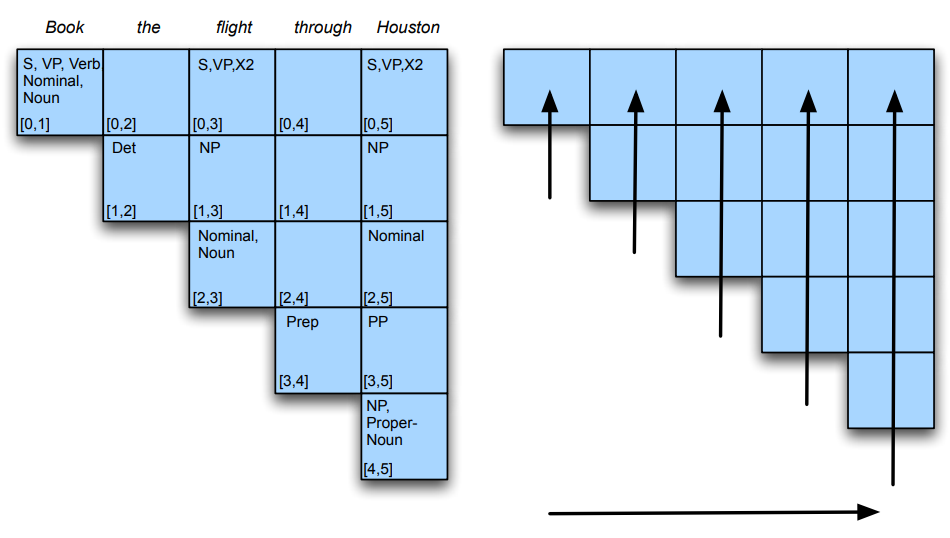
\includegraphics[width=0.85\linewidth]{images/Cocke_DP_Algo.png}
	\caption{Пример заполнения таблицы для предложения <<Book the flight through Houston>>}
	\label{fig:cocke_Algo}
\end{figure}

Заполнен	ие таблицы $dp$ производится слева направо, снизу-вверх, к моменту вычисления $dp_{i,\ j}$ известны значения всех $dp_{l,\ j},\ l<i$ и $dp_{i,\ m},\ m<j$, соответственно могут быть проверены все возможные разбиения интервала $[i, j]$. Варианты разбора входного предложения, таким образом, находятся в $dp_{0,\ n}$. Выбор верного варианта разбора среди представленных в $dp_{0,\ n}$ осуществляется вручную или предобученным классификатором.

Для построения дерева составляющих по заполненной таблице $dp$ при добавлении $A$ в $dp_{i,j}$ из правила $A \to B\,C$ и разбиения $k$ сохраняют указатели на $dp_{i,k}$ и $dp_{k,j}$ и использованное правило. Восстановление дерева --- рекурсивный обход от выбранного $S \in dp_{0,n}$. При нескольких разборах выбор одного дерева выносится за рамки классического CYK и может выполняться вручную, по дополнительным ограничениям грамматики или с помощью предобученной модели, оценивающей правдоподобность конституент~\cite{jurafsky2026speech}.


Вычислительная сложность распознавания для грамматики фиксированного размера составляет $O(n^3)$ при длине предложения $n$~\cite{makarov2022cockeyoungerkasamischwartzzippelalgorithmrelatives}.

\subsection{Алгоритм Эрли}
Алгоритм Эрли~\cite{earley1970efficient,jurafsky2026speech} относится к методам синтаксического разбора контекстно-свободных грамматик также с использованием подхода динамического программирования. 

Для предложения из $n$ словоформ данный алгоритм формирует массив $dp$ множеств состояний размера $n+1$. $dp_i$ соответствует множеству возможных состояний частично построенного дерева зависимостей после обработки $i$ словоформ. При этом в ходе работы, алгоритм совершает единственный обход предложения слева-направо, не обрабатывая повторно уже полученные составляющие. 

Состояние описывается тройкой вида~\ref{eq:early_state}:

\begin{equation}
	\label{eq:early_state}
	\langle r,\ p,\ [i,j]\rangle,
\end{equation}
\noindent\makebox[0pt][l]{где }\hspace*{\parindent}$r$~---~правило контекстно-свободной грамматики вида $A \rightarrow (X_1,\ X_2,\ \ldots\ X_m)$;

$p \in \overline{0,m}$~---~позиция отметки в правой части правила $r$;

$[i, j],\ 0\le i\le j \le n$~---~границы фрагмента исходного предложения, соответствующие правой части правила $r$, расположенной до метки $p$.

Начальное состояние разбора описывается тройкой~\ref{eq:early_start_state} и помещается в множество состояний $dp_0$ до начала работы алгоритма.
\begin{equation}
	\label{eq:early_start_state}
	\langle \gamma \rightarrow S,\; 0,\; [ 0,0]\rangle,
\end{equation}
\noindent\makebox[0pt][l]{где }\hspace*{\parindent}$\gamma$ --- вспомогательный нетерминал;

$S$ --- стартовый символ грамматики.

Предложение из $n$ словоформ считается успешно разобранным в случае, если тройка~\ref{eq:early_end_state} находится в множестве состояний $dp_n$.
\begin{equation}
	\label{eq:early_end_state}
	\langle \gamma \rightarrow S,\ 1,\ [ 0,n]\rangle
\end{equation}

Обработка префикса предложения из $i$ словоформ заключается в обходе каждого состояния множества $dp_i$ и применения ровно одной из трёх нижеописанных операций в зависимости от состояния, либо пропуска данного состояния в случае неприменимости ни одной из операций. Полученные в результате применения операций новые состояния добавляются в $dp_{i}$ или $dp_{i+1}$.

Алгоритм Эрли использует следующие операции для обработки состояний в $dp$:
\begin{itemize}
	\item операция предсказания (predictor);
	\item операция чтения терминала (scanner);
	\item операция завершения разбора правила (completer).
\end{itemize}

Операция предсказания применяется в случае, если в $dp_j$ обрабатывается состояние $\langle A \rightarrow X_1,\ \ldots\ X_p,\ X_{p+1},\ \ldots\ X_m,\ p,\ [i, j]\rangle$ и $X_{p+1}$ является нетерминалом. Для каждого правила грамматики вида $X_{p+1} \rightarrow Y_1,\ \ldots\ Y_l$ в $dp_j$ добавляют состояния $\langle X_{p+1} \rightarrow Y_1,\ \ldots\ Y_l,\ 0,\ [j, j]\rangle$. При этом операция предсказания не изменяет $j$, то есть длина обработанного префикса предложения не изменяется.

Операция чтения терминала применяется в случае, если в $dp_j$ обрабатывается состояние $\langle A \rightarrow X_1,\ \ldots\ X_p,\ X_{p+1},\ \ldots\ X_m,\ p,\ [i, j]\rangle$ и $X_{p+1}$ и $X_{p+1}$ является терминалом, и словоформа на позиции $j+1$ удовлетворяет данному терминалу. В результате применения операции чтения терминала в $dp_{j+1}$ добавляется состояние $\langle A \rightarrow X_1,\ \ldots\ X_m,\ p+1, [i, j+1]\rangle$. Таким образом, операция чтения терминала сдвигает метку $p$ в правиле $r$ на единицу вправо, и увеличивает длину разобранного фрагмента предложения также на единицу.

Операция завершения разбора правила применяется в случае, если в $dp_j$ обрабатывается состояние $\langle A \rightarrow X_1,\ \ldots\ X_p,\ X_{p+1},\ \ldots\ X_m,\ m,\ [i, j]\rangle$, т.~е. нетерминал $A$ полностью разобран на интервале $[j, j]$. Для каждого состояния в $dp_i$ вида $\langle B \rightarrow Y_1,\ \ldots\ Y_{t},\ A,\ Y_{t+2},\ \ldots\ Y_l, t, [k, i] \rangle$ в $dp_j$ добавляют состояния $\langle B \rightarrow Y_1,\ \ldots\ Y_{t},\ A,\ Y_{t+2},\ \ldots\ Y_l, t+1, [k, j] \rangle$. Таким образом, операция завершения разбора правила изменяет отметку $p$ в правилах для нетерминала $B$ и увеличивая интервал действия до $j$.

В худшем случае время работы алгоритма Эрли оценивается как $O(n^3)$ при длине предложения $n$; для многих однозначных грамматик на практике наблюдается поведение ближе к $O(n^2)$~\cite{earley1970efficient,jurafsky2026speech}.

\subsection{Сравнение методов построения систем составляющих}

Для сравнения алгоритмов CYK и Эрли выделены следующие критерии:
\begin{itemize}
	\item вычислительная сложность алгоритмов в худшем случае;
	\item необходимость предварительного приведения к нормальной форме Хомского;
	\item максимальная длина правой части правила в грамматике;
	\item число параметров необходимых для разбора подотрезка предложения;
	\item число типов операций для построения составляющей;
	\item оценка числа состояний в худшем случае;
	\item оценка необходимой памяти в худшем случае;
	\item возможность построения span-таблицы синтаксических единиц предложения;
	\item возможность вероятностного выбора синтаксической единицы для разрешения неоднозначности разбора.
\end{itemize}

Сравнение в соответствии с сформулированными критериями приведено в таблице~\ref{tab:cyk_earley}.

\begin{table}[H]
	\centering
	\caption{Сравнение алгоритмов CYK и Эрли}
	\label{tab:cyk_earley}
	\small
	\begin{tabular}{|p{5.8cm}|p{2cm}|p{2cm}|p{5.2cm}|}
		\hline
		Критерий & Алгоритм CYK & Алгоритм Эрли & Примечание \\
		\hline
		Вычислительная сложность в худшем случае & $O(n^3)$ & $O(n^3)$ & На основе~\cite{younger1967recognition,earley1970efficient} \\
		\hline
		Требуется предварительное приведение к НФХ & Да & Нет & Вид правил алгоритма CYK: $A\to BC$ или $A\to w$ \\
		\hline
		Максимальная длина правой части правила без преобразования & 2 & Не ограничена &  \\
		\hline
		Число параметров, определяющих разбор подотрезка предложения & 2 & 3 & Алгоритм CYK: $(i,j)$, $0\le i<j\le n$ \newline Алгоритм Эрли: $(r,p,[i,j])$  \\
		\hline
		Число типов операций для построения составляющей & 1 & 3 & \\
		\hline
		Оценка числа состояний, худший случай & $O(n^2|N|)$ & $O(n^3|P|)$ & $|N|$~---~число различных нетерминалов в грамматике\newline $|P|$~---~число правил в грамматике\\
		\hline
		Оценка памяти в худшем случае & $O(n^2)$ & $O(n^3)$ & На основе~\cite{jurafsky2026speech,earley1970efficient,makarov2022cockeyoungerkasamischwartzzippelalgorithmrelatives}\\
		\hline
		Построение span-таблицы всех синтаксических единиц предложения & Да & Нет &  \\
		\hline
		Возможность вероятностного выбора синтаксической единицы для разрешения неоднозначности разбора & Да & Да & \\
		\hline
	\end{tabular}
\end{table}

В соответствии с представленным сравнением алгоритм CYK является более предпочтительным для реализации метода построения деревьев составляющих для ограниченного естественного русского языка в связи с: 
\begin{itemize}
	\item более полным соответствием формализму деревьев составляющих, как множеству непересекающихся, либо вложенных подотрезков предложения;
	\item меньшими затратами памяти, числом состояний и параметров;
	\item возможностью построения span-таблицы всех синтаксических единиц предложения с целью дальнейшего анализа их употребимости.
\end{itemize}

\section{Постановка задачи}

Для реализации метода построения синтаксических деревьев ограниченного естественного русского языка необходимо определить:
\begin{itemize}
	\item определить формат входных и выходных данных;
	\item определить правила грамматики применяемые в ограниченном русском языке;
	\item определить типы согласования применяемые в ограниченном русском языке;
	\item определить необходимые морфологические характеристики словоформ.
\end{itemize}

Метод построения синтаксических деревьев для ограниченного естественного русского языка принимает предложение в виде последовательности словоформ. Метод возвращает размеченное дерево составляющих, вершины которого содержат метки синтаксических единиц в вершинах имеющих потомков, словоформы в листовых вершинах.

Наиболее употребимые в ограниченном естественном русском языке правила грамматики~\cite{syntagrus_syntax_annotation,Testelets2001} представлены в приложении Б. Наиболее употребимые~\cite{syntagrus_syntax_annotation,Testelets2001} правила согласования приведены в приложении B. Для использования правил согласования и грамматики необходимы следующие морфологические характеристики:
\begin{itemize}
	\item существительное: род, число, падеж;
	\item прилагательное и причастие: род, число, падеж;
	\item глагол в личной форме: время, число, лицо, переходность;
	\item глагол в инфинитиве: переходность;
	\item местоимение: род, число, падеж, лицо;
	\item числительное: тип, падеж, число, род.
\end{itemize}
Для наречий, деепричастий, предлогов, союзов, частиц определяется только часть речи. При этом для предлогов необходимо указать падеж, который должно принимать существительное, согласующееся с данным предлогом.

Формализованная постановка задачи в виде функциональной модели в нотации IDEF0 представлена на рисунках~\ref{fig:idef0_A0},~\ref{fig:idef0_A1}.

\begin{figure}[H]
	\centering
	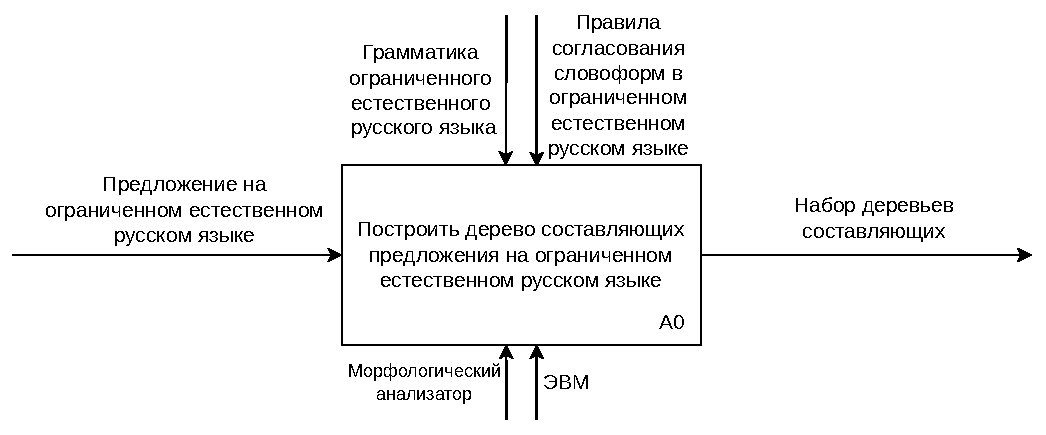
\includegraphics[width=0.8\linewidth]{images/A0.pdf}
	\caption{IDEF0-диаграмма уровня A0}
	\label{fig:idef0_A0}
\end{figure}

\begin{figure}[H]
	\centering
	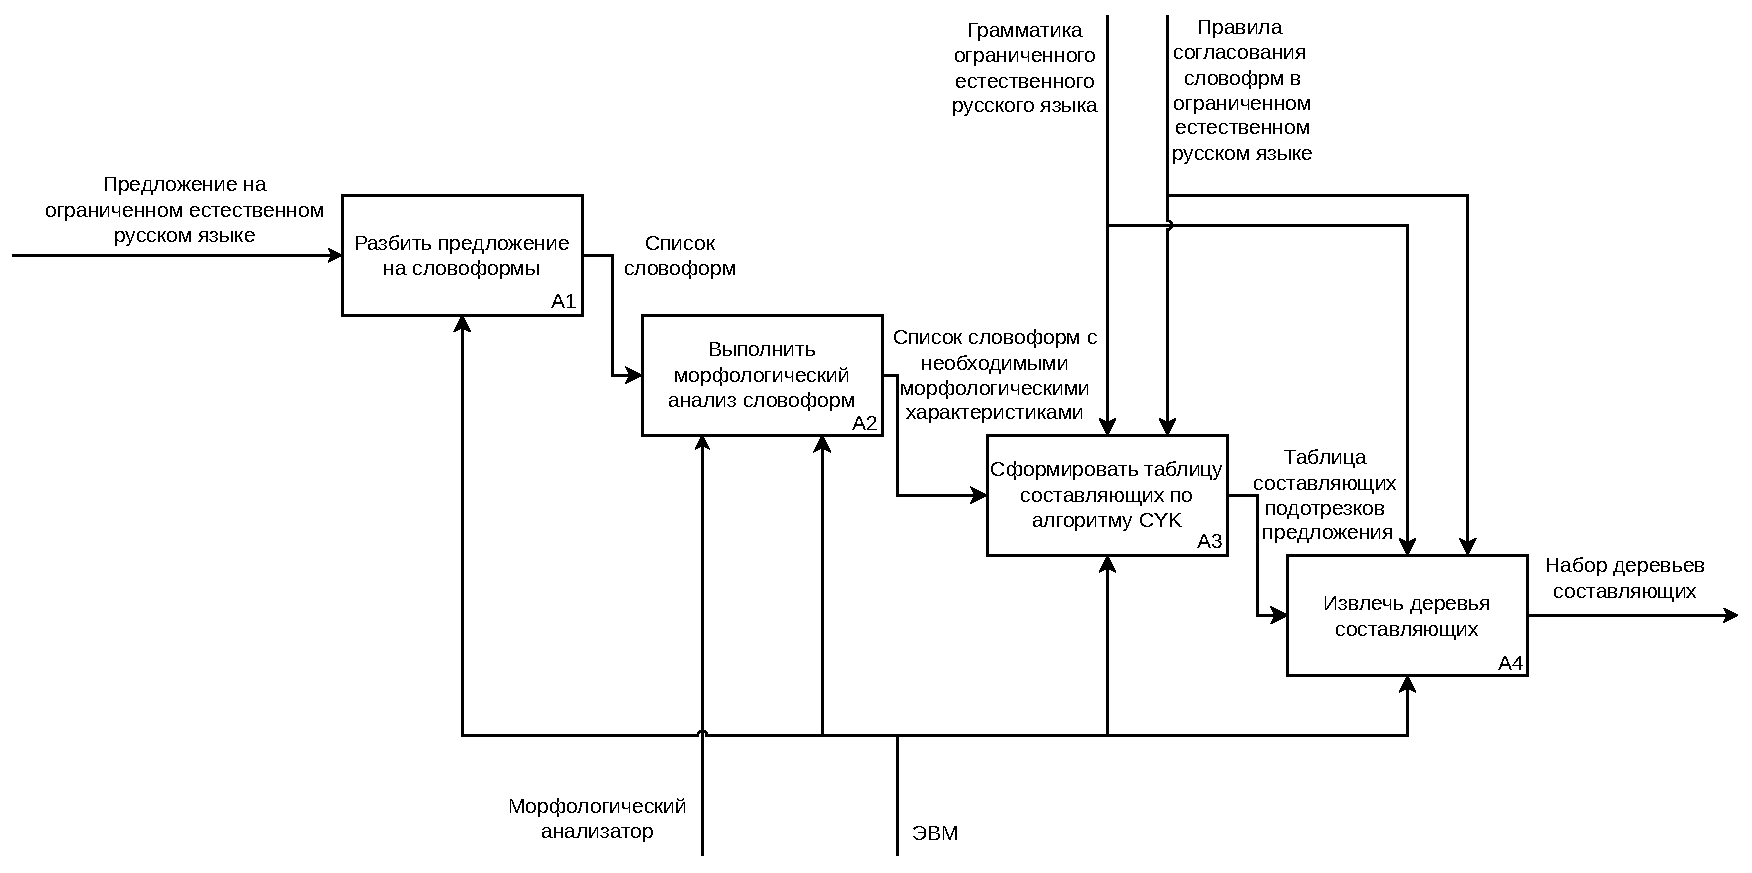
\includegraphics[width=\linewidth]{images/A1.pdf}
	\caption{IDEF0-диаграмма уровня A1}
	\label{fig:idef0_A1}
\end{figure}

\section*{Выводы}

В данном разделе введены основные понятия предметной области автоматизированной синтаксической разметки ограниченного естественного русского языка, описаны системы синтаксической разметки. Приведено сравнение данных систем. Описаны существующие методы построения систем составляющих, приведено их сравнение. Определены формат входных и выходных данных метода построения деревьев составляющих, описаны наиболее употребимые правила грамматики и согласования, выделены необходимые для их использования морфологические характеристики словоформ. Приведена формализованная постановка задачи в нотации IDEF0.
